%\documentclass[a4paper,12pt]{article}  % standard LaTeX, 12 point type
\documentclass[12pt, a4paper]{article}

\usepackage{algpseudocode}
\usepackage{algorithm}
\usepackage{algorithmicx}

\usepackage{proof}
\usepackage{stmaryrd}

\usepackage{geometry}
\usepackage{amsfonts,latexsym}
\usepackage{amsthm}
\usepackage{amssymb}
\usepackage[utf8]{inputenc} % Кодировка
\usepackage[english,russian]{babel} % Многоязычность
\usepackage{mathtools}
\usepackage{hyperref}
\usepackage{tikz}
\usepackage{dsfont}
\usepackage{multicol}
\usetikzlibrary{fit,calc,automata,positioning}

\theoremstyle{definition}
\newtheorem{definition}{Определение}[section]
\newtheorem{example}{Пример}[section]
\newtheorem{theorem}{Теорема}[section]
\newtheorem{proposition}[theorem]{Proposition}
\newtheorem{lemma}[theorem]{Лемма}
\newtheorem{corollary}[theorem]{Corollary}
\newtheorem{conjecture}[theorem]{Conjecture}


% unnumbered environments:

\theoremstyle{remark}
\newtheorem*{remark}{Remark}
\newtheorem*{notation}{Notation}
\newtheorem*{note}{Note}



\setlength{\parskip}{5pt plus 2pt minus 1pt}
%\setlength{\parindent}{0pt}


\algtext*{EndWhile}% Remove "end while" text
\algtext*{EndIf}% Remove "end if" text
\algtext*{EndFor}% Remove "end for" text
\algtext*{EndFunction}% Remove "end function" text


\usepackage{color}
\usepackage{listings}
\usepackage{caption}
\usepackage{graphicx}
\usepackage{ucs}

\graphicspath{{pics/}}

\geometry{left=2cm}
\geometry{right=1.5cm}
\geometry{top=2cm}
\geometry{bottom=2cm}




%\lstnewenvironment{algorithm}[1][]
%{
%    \lstset{
%        frame=tB,
%        numbers=left,
%        mathescape=true,
%        numberstyle=\small,
%        basicstyle=\small,
%        inputencoding=utf8,
%        extendedchars=\true,
%        keywordstyle=\color{black}\bfseries,
%        keywords={,function, procedure, return, datatype, function, in, if, else, for, foreach, while, denote, do, and, then, assert,}
%        numbers=left,
%        xleftmargin=.04\textwidth,
%        #1 % this is to add specific settings to an usage of this environment (for instnce, the caption and referable label)
%    }
%}
%{}

\newcommand{\tab}[1][0.3cm]{\ensuremath{\hspace*{#1}}}

\newcommand{\rvline}{\hspace*{-\arraycolsep}\vline\hspace*{-\arraycolsep}}

\newcommand{\derives}[1][*]{\xRightarrow[]{#1}}
\newcommand{\first}[1][1]{\textsc{first}_{#1}}
\newcommand{\follow}[1][1]{\textsc{follow}_{#1}}

\setcounter{MaxMatrixCols}{20}


\tikzset{
%->, % makes the edges directed
%>=stealth’, % makes the arrow heads bold
node distance=4cm, % specifies the minimum distance between two nodes. Change if necessary.
%every state/.style={thick, fill=gray!10}, % sets the properties for each ’state’ node
initial text=$ $, % sets the text that appears on the start arrow
}

\tikzstyle{symbol_node} = [shape=rectangle, rounded corners, draw, align=center]
\tikzstyle{prod_node} = [shape=rectangle, draw, align=center]

\tikzset{
    between/.style args={#1 and #2}{
         at = ($(#1)!0.5!(#2)$)
    }
}

%every node/.style = {shape=rectangle, rounded corners,
%      draw, align=center,
%      top color=white, bottom color=blue!20}

\title{Теория формальных языков. Лекции и практики. Заметки.}
\author{Семён Григорьев}
\date{\today}

\begin{document}
\maketitle
\newpage
\tableofcontents
\newpage

\section{Правила работы на курсе}

Коротко зафиксируем основные правила работы на курсе: из чего формируется оценка, как сдавать домашние работы и т.д.

\subsection{Оценка за курс}

Оценка за курс складывается из баллов, полученных за работу в семестре. Баллы начисляются за следующее.
\begin{itemize}
    \item За домашние работы (балл за каждую задачу указывается отдельно). При этом у каждой работы есть жёсткий дедлайн и после него балл уменьшается вдвое.
    \item За летучки (короткие, 5-10 минут, контрольные работы). Летучка оценивается от 1 до 0 баллов с шагом 0.25. Сами по себе баллы за летучки не суммируются, но служат для корректировки баллов за домашние работы.
\end{itemize}

Итоговая оценка за курс --- это взвешенная сумма баллов за задачи, где вес --- баллы за ближайшую справа летучку.
Пусть, например, в курсе было 4 задачи и 2 летучки, упорядоченны хронологически как это показано в таблице~\ref{tbl:grad_example}.
В этой же таблице можно увидеть, какие баллы получил Эталон Примерович за задачи и летучки, а также его итоговый балл, который вычисляется следующим образом:
$$
\underbrace{(4+5)}_{\text{Первые две домашки}}*\underbrace{0.25}_{\text{Летучка 1}} + \underbrace{(2.5+3)}_{\text{Вторые две домашки}}*\underbrace{0.75}_{\text{Летучка 2}} = 6.375.
$$

\begin{table}[h]
    \caption{Пример оценок за курс}
    \label{tbl:grad_example}
\begin{center}
    \begin{tabular}{ | c | c | c | c | c | c | c | c |}
        \hline
        ФИО & ДЗ 1 & ДЗ 2 & Летучка 1 & ДЗ 3 & ДЗ 4 & Летучка 2 &  Итог \\
        \hline
        \hline
        Эталон Примерович & 4 & 5 & 0.25 & 2.5 & 3 & 0.75 & 6.375 \\
        \hline
    \end{tabular}
\end{center}
\end{table}


Для трансляции баллов в оценку используется таблица~\ref{tbl:ects}.

\begin{table}[h]
    \caption{Конвертация баллов в оценки}
    \label{tbl:ects}
\begin{center}
    \begin{tabular}{ | c | c | c |}
        \hline
        Балл & ECTS & Классика \\
        \hline
        \hline
        91--100 & A & 5 \\
        81--90  & B & 4 \\
        71--80  & C & 4 \\
        61--70  & D & 3 \\
        51--60  & E & 3 \\
         0--50  & F & 2 \\
        \hline
    \end{tabular}
\end{center}
\end{table}

Решение задач можно продолжать до тех пор, пока не будет набрано достаточно баллов для получения неотрицательной оценки (с учётом понижения баллов после дедлайнов и с учётом летучек\footnote{Поэтому летучки имеет смысл писать всегда. Они могут влияют на задачи, даже если те сданы после написания летучки.}).
Если даже при всех решённых задачах баллов не достаточно для получения неотрицательной оценки, то выдаются дополнительные задачи\footnote{Дополнительные задачи выдаются только после решения основных.}.
Баллы за дополнительные задачи таковы, чтобы обеспечить разве что получение минимальной положительной оценки.

Все текущие результаты оформляются в виде таблицы на Google Drive.
Таблица доступна всем студентам на чтение.

\subsection{Домашние задачи}

Домашние задачи представляют из себя практические задачи на программирование или постановку экспериментов (сравнение и анализ производительности различных алгоритмов, решений).
Они анонсируются по ходу семестра вместе с баллами и дедлайнами.
У задачи есть два дедлайна: \textbf{мягкий} и \textbf{жёсткий}.
\textbf{Мягкий} наступает через 4 дня после выдачи задачи (если не оговорено иное) и нужен для того, чтобы гарантировать своевременную проверку задачи.
Задача, ревью на которую запрошено до мягкого дедлайна гарантированно будет проверена с возможностью исправить замечания до наступления жёсткого дедлайна. Если задача сдана после мягкого дедлайна, то своевременность проверки уже не гарантируется. То есть возможны следующие ситуации/
\begin{itemize}
    \item Задача сразу решена правильно и тогда не зависимо от времени проверки за неё даётся полный балл
    \item Задача решена не правильно но проверена и исправлена до жёсткого дедлайна. Тогда получается полный балл. Но, как было сказано выше, нет гарантии, что хватит времени на исправление.
    \item Задача решена не правильно и это выяснилось после жёсткого дедлайна: тогда за неё уже нельзя получить полный балл.
\end{itemize}
\textbf{Жёсткий} дедлайн не может наступить раньше, чем через 6 дней с момента анонса задачи, как правило равен неделе, но может быть и больше. После жёсткого дедлайна баллы разово снижаются в два раза\footnote{То есть задача, сданная в любой момент после жёсткого дедлайна стоит в два раза меньше, чем сданная вовремя. Судя по всему, Эталон Примерович из таблицы~\ref{tbl:grad_example} сдал задачу 3 после жёсткого дедлайна.}. Любая задача может быть либо зачтена полностью, либо не зачтена вообще\footnote{То есть частично решённых задач быть не может. А значит, и неполных баллов.}. Полный балл за все задачи --- 100.
Каждый раз задаётся (и, соответственно, сдаётся) одна задача\footnote{Таким образом, идеальный расклад --- одна задача в неделю. На некоторые задачи, правда, может выделяться больше времени.}.

Язык программирования --- Python. Набор инструментов и структура репозитория для домашних задач фиксированы и представлены здесь: \url{https://github.com/JetBrains-Research/formal-lang-course}.
Набор библиотек следующий.
\begin{itemize}
    \item cfpq\_data для работы со входными данными (графами).
    \item sciPy для базовых операций с матрицами.
    \item pygraphblas для оптимизированных операций с матрицами на CPU.
    \item pyspbla (pycubool?) для булевых матриц на GPU.
    \item pyformlang для работы с языками (регулярные выражения, конечные автоматы, КС грамматики).
    \item ANTLR для синтаксического анализа.
    \item pyTest для организации тестов.
    \item pyDOT для визуализации графов.
\end{itemize}

Так как часть задач будет состоять в постановке экспериментов, то для них требуется оформление отчёта по поставленным экспериментам.
Отчёт оформляется как Python notebook в Google Colab, который содержит как код для постановки экспериментов (чтобы было видно, что и как замеряли), так и весь сопроводительный текст, графики и т.д.

Качество оформления отчёта влияет на то, будет ли зачтена задача. То есть, даже если всё замерено грамотно, но отчёт оформлен небрежно, то задача может быть не зачтена.

Задачи сдаются через GitHub. Процедура выглядит следующим образом.
\begin{enumerate}
    \item Студент создаёт репозиторий, в который приглашает ассистентов, помогающих с проверкой домашних заданий (анонсируются на первой паре). Запись об этом репозитории добавляется в таблицу с результатами.
    \item Студенты распределяются преподавателем среди ассистентов.
    \item Репозиторий снабжается readme, системой автоматической сборки, системой автоматического тестирования, проверкой качества кода. Для упрощения этого шага необходимо пользоваться предоставленным шаблоном: достаточно сделать его fork.
    \item Новая задача решается в отдельной ветке. Если это задача на постановку экспериментов, то ссылка на notebook добавляется в readme репозитория. При решении задачи необходимо следовать структуре, заданной в репозитории-шаблоне. Задача снабжается тестами. Качество тестов --- обязанность студента. Задача может быть не принята из-за плохого тестового покрытия. После того, как все автоматические проверки пройдены, открывается реквест в основную ветку. Если и реквест прошёл все автоматические проверки, то запрашивается ревью у соответствующего ассистента\footnote{Запрос ревью --- есть попытка сдачи, которая регламентируется дедлайнами. Запрашивать ревью можно только на полностью решённую задачу. Нельзя запрашивать ревью на частичные решения.}.
    \item Ассистент выполняет проверку, оставляет комментарии, выносит вердикт. Если задача зачтена, то реквест мёржится и закрывается студентом, а балл за задачу заносится в таблицу ассистентом. Иначе вносятся исправления, добавляются к этому же реквесту\footnote{Реквест не закрывать. Это позволяет отслеживать историю замечаний.}, заново запрашивается ревью\footnote{Запрашивать ревью обязательно, так как каждый коммит проверять никто не будет.}. и так до тех пор, пока задача не будет зачтена\footnote{Ну, или до тех пор, пока не отпадёт необходимость её решать.}.
\end{enumerate}

Необходимо иметь ввиду, что многие задачи связаны между собой (следующая использует результаты предыдущих), поэтому не всегда возможно безболезненно не делать какую-то одну задачу из середины списка.

\subsection{Летучки}

Летучка --- небольшая, на 5--10 минут, проверочная работа, проводимая в начале пары.
Летучка проверяет базовые знания: определения, теоремы, алгоритмы, свойства алгоритмов.
Она содержит одно задание, которое может быть как теоретическим (написать определение чего либо), так и практическим (показать шаги какого-то алгоритма для заданного входа).

Летучка оценивается от 0 до 1 балла с шагом в 0.25 и используется как вес для домашних работ. Оценки летучек не обсуждаются и не корректируются. Летучки не переписываются.

Точная дата летучки заранее не анонсируется, однако их примерное местоположение может быть известно заранее, так как обычно они привязываются к тем или иным блокам материала.

Точное количество летучек также заранее не известно, но обычно это 4--5. Так как могут быть уважительные причины пропустить летучку, то в конце семестра за две случайно выбранные летучки с нулём баллов выставляется 0.75 баллов\footnote{Просто чтобы написать самому было лучше, чем прогулять и понадеяться на случайность.}.

При занятиях в аудитории летучка пишется на листке бумаги, на котором, кроме решения задач, указывается ФИО студента и вариант (который назначается преподавателем). Листочки сдаются строго по истечению отведённого времени.

При занятии в удалённом формате всё происходит точно также, только сдаётся фотография (скан) листочка. Способ сдачи указывается преподавателем перед началом летучки. Время необходимое на отправку фото входит во время всей летучки\footnote{Так что будьте осторожны. Если на летучку дали 10 минут, то через 10 минут фото листочка должно быть у преподавателя. А не через 10 минут срочно начнётся поиск внезапно пропавшего телефона и т.д.}.

Примеры вопросов на летучку.
\begin{enumerate}
    \item Какова сложность алгоритма Хеллингса относительно размера графа?
    \item В чём отличие НФХ от ОНФХ?
    \item Дайте определение рекурсивного конечного автомата.
    \item Нарисуйте начальное состояние таблицы CYK для данного входа и грамматики.
    \item Принимается ли данная цепочка данным автоматом? Если да, то предъявите соответствующую последовательность переходов.
    \item Какова сложность тензорного произведения относительно размера исходных матриц?
\end{enumerate}


\section{План занятий}
\begin{enumerate}
  \item Введение. О чём курс: общая структура, что будет и чего не будет. Правила получения оценки за курс. Базовые определения.
  \item Иерархия Хомского. Основные классы языков. За пределами иерархии Хомского. Нестроковые языки.
  \item Задача поиска пути с ограничениями в терминах формальных языков. Варианты постановки, прикладное значение, теоретические вопросы.
  \item Регулярные языки, конечные автоматы (детерминированные, недетерминированные), регулярные выражения. Операции над ними. Операции над автоматами как операции над их матрицами смежности. Поиск путей с регулярными ограничениями.
  \item Контекстно-свободные языки. Нормальная и ослабленная нормальная формы Хомского. Поиск путей с КС ограничениями. CYK и Hellings.
  \item Матричный алгоритм КС запросов.
  \item Тензорный алгоритм КС запросов.
  \item Дерево разбора и поиск путей. SPPF.
  \item Синтаксический анализ языков программирования. Лексика и синтаксис. Тонкости, проблемы, инструменты.
  \item ANTLR, LL, ещё раз про неоднозначности.
  \item Семантика языков программирования. Интерпретаторы. Что делать с деревом разбора.
  \item Атрибутные грамматики.
  \item Немного о том, что за КС тоже есть жизнь.
\end{enumerate}


Общая цель курса --- посмотреть на формальные языки с прикладной точки зрения. При этом предлагается попробовать применить их сразу в двух областях: классический синтаксический анализ языков программирования и анализ графов.

В ходе курса будет предложено разработать небольшой инструментарий для выполнения запросов к графам. Окажется, что алгоритмы для некоторых задач анализа графов непосредственно основаны на алгоритмах из теории формальных языков и синтаксического анализа. Далее, будет предложено разработать язык запросов, позволяющий использовать разработанные алгоритмы. Необходимо будет разработать сам язык, лексический и синтаксический  анализаторы для него, интерпретатор. Интерпретатор будет использовать разработанные алгоритмы выполнения запросов к графам.

Таким образом, в результате работы над задачами у каждого должно получиться приложение, предоставляющее REPL для работы с графами, поддерживающее следующие возможности (список может дополняться). 
\begin{enumerate}
\item Проверить, какие графы доступны.
\item Узнать базовую информацию о выбранных графах (количество вершин, рёбер, метки на рёбрах и т.д.).
\item Сгенерировать синтетический граф.
\item Описать запрос.
\item Задать запрос к некоторым графам.
\end{enumerate}
В качестве примера можно ориентироваться на SQL-консоль.

Гипотетический пример работы:
\begin{verbatim}
  GQL> list graphs
  geospecies
  fof
  drivers
  GQL> list labels 'fof'
  l1
  l2
  GQL> let S = l1 S l2 | eps
  S: constraint
  GQL> select v1,v2 from 'fof' where v1 -S-> v2
  0, 10
  2, 9
  ....
\end{verbatim}


Примерные темы задач с баллами.
\begin{enumerate}
  \item [5] Развернуть репозиторий, снабдить его всем необходимым (сборка, тесты). Научиться подгружать графы из набора данных, запрашивать у них вершины и рёбра. На основе этой функциональности реализовать первые тесты. Реализовать консольный интерфейс, позволяющий получить количество вершин и рёбер для указанного графа. Далее этот интерфейс будет расширяться и остальные задачи должны уметь работать с консолью.
  \item [2] Реализовать преобразование регулярного выражения в ДКА.
  \item [2] Реализовать преобразование графа в НКА.
  \item [5] Реализовать алгоритм выполнения регулярных запросов через тензорное произведение.
  \item [11] Сравнение производительности пересечения автоматов через тензорное произведение и стандартное из Pyformlang.
  \item [2] Реализовать преобразование контекстно-свободной грамматики в НФХ и ОНФХ.
  \item [5] Реализовать построение рекурсивного конечного автомата и его минимизацию.
  \item [5] Реализовать алгоритм синтаксического анализа CYK.
  \item [5] Реализовать алгоритм Хеллингса для задачи достижимости с контекстно-свободными ограничениями.
  \item [5] Реализовать матричный алгоритм (для булевых матриц) для задачи достижимости с контекстно-свободными ограничениями.
  \item [5] Реализовать тензорный алгоритм (для булевых матриц) для задачи достижимости с контекстно-свободными ограничениями.
  \item [15] Сравнение производительности алгоритмов для задачи достижимости с контекстно-свободными ограничениями: Хеллингс, матричный, тензорный.
  \item [5] Разработать конкретный синтаксис языка запросов к графам. Описать его в виде документации в репозитории. Снабдить примерами
  \item [5] Реализовать его парсер языка запросов к графам, согласно разработанному синтаксису.
  \item [3] Реализовать печать дерева разбора в DOT на основе стандартных возможностей ANTLR.
  \item [20] Реализовать интерпретатор языка запросов к графам.
\end{enumerate}


\section{Лекция 1: Введение}

Алфавит, язык. Операции над строками. Операции над языками.

Какие вопросы можно задавать о языках: о пустоте, универсальности, о построении пересечения, о пустоте пересечения, о вложенности, об эквивалентности.

Базовые способы задания: перечисление, генератор, распознаватель.

Взаимосвязь теории формальных языков с другими областями, области её применения.
\begin{itemize}
  \item Синтаксический анализ языков программирования: в компиляторах, интерпертаторах, средах разработки, других инстументах.
  \item Анализ естественных языков.
  Активность в этой области несколько спала, так как на передний план сейчас вышли различные методы машинного обучения.
  Однако и в этой области ведуться работы.
  Примеры конференций:
  \begin{itemize}
    \item \href{http://www.wikicfp.com/cfp/servlet/event.showcfp?eventid=98626&copyownerid=320}{International Conference on Parsing Technologies} (\href{https://iwpt20.sigparse.org/callforpapers.html}{IWPT-2020})
    \item \href{http://www.wikicfp.com/cfp/program?id=1029&s=FG&f=Formal%20Grammar}{FG: Formal Grammar} (\href{http://fg.phil.hhu.de/2020/}{FG-2020})
  \end{itemize}

  \item Статический анализ кода.
  \begin{itemize}
    \item Различные задачи межпроцедурного анализа. Основной подход --- language reachability. Основоположник --- Томас Репс. Примеры работ.
    \begin{itemize}
      \item Thomas Reps. 1997. Program analysis via graph reachability. In Proceedings of the 1997 international symposium on Logic programming (ILPS ’97). MIT Press, Cambridge, MA, USA, 5–19.
      \item Qirun Zhang and Zhendong Su. 2017. Context-sensitive data-dependence analysis via linear conjunctive language reachability. In Proceedings of the 44th ACM SIGPLAN Symposium on Principles of Programming Languages (POPL 2017). Association for Computing Machinery, New York, NY, USA, 344–358. DOI:https://doi.org/10.1145/3009837.3009848
      \item Kai Wang, Aftab Hussain, Zhiqiang Zuo, Guoqing Xu, and Ardalan Amiri Sani. 2017. Graspan: A Single-machine Disk-based Graph System for Interprocedural Static Analyses of Large-scale Systems Code. In Proceedings of the Twenty-Second International Conference on Architectural Support for Programming Languages and Operating Systems (ASPLOS ’17). Association for Computing Machinery, New York, NY, USA, 389–404. DOI:https://doi.org/10.1145/3037697.3037744
      \item Lu Y., Shang L., Xie X., Xue J. (2013) An Incremental Points-to Analysis with CFL-Reachability. In: Jhala R., De Bosschere K. (eds) Compiler Construction. CC 2013. Lecture Notes in Computer Science, vol 7791. Springer, Berlin, Heidelberg
    \end{itemize}
    \item Интерливинг (или шафл) языков для верификаци многопоточных программ.
    \begin{itemize}
      \item \href{http://uu.diva-portal.org/smash/get/diva2:442518/FULLTEXT01.pdf}{Approximating the Shuffle of Context-free Languages to Find Bugs in Concurrent Recursive Programs}
      \item Flick N.E. (2015) Quotients of Unbounded Parallelism. In: Leucker M., Rueda C., Valencia F. (eds) Theoretical Aspects of Computing - ICTAC 2015. ICTAC 2015. Lecture Notes in Computer Science, vol 9399. Springer, Cham
    \end{itemize}

    \item Система типов Java: \href{https://arxiv.org/abs/1605.05274}{Radu Grigore, Java Generics are Turing Complete}.
  \end{itemize}

  \item Графовые базы данных. Поиск путей с ограничениями.
    \begin{itemize}
      \item Maurizio Nolé and Carlo Sartiani. 2016. Regular Path Queries on Massive Graphs. In Proceedings of the 28th International Conference on Scientific and Statistical Database Management (SSDBM ’16). Association for Computing Machinery, New York, NY, USA, Article 13, 1–12. DOI:https://doi.org/10.1145/2949689.2949711
      \item Jochem Kuijpers, George Fletcher, Nikolay Yakovets, and Tobias Lindaaker. 2019. An Experimental Study of Context-Free Path Query Evaluation Methods. In Proceedings of the 31st International Conference on Scientific and Statistical Database Management (SSDBM ’19). Association for Computing Machinery, New York, NY, USA, 121–132. DOI:https://doi.org/10.1145/3335783.3335791
      \item \href{https://arxiv.org/abs/1502.02242}{Jelle Hellings. Querying for Paths in Graphs using Context-Free Path Queries.}
    \end{itemize}

  \item Биоинформатика. В основном это анализ геномных и белковых последовательностей.
    \begin{itemize}
      \item \href{https://www.ncbi.nlm.nih.gov/pmc/articles/PMC6428041/}{Witold Dyrka, Mateusz Pyzik, Francois Coste, and Hugo Talibart. Estimating probabilistic context-free grammars for proteins using contact map constraints}.
      \item \href{https://www.ncbi.nlm.nih.gov/pmc/articles/PMC3464655/}{James WJ Anderson, Paula Tataru, Joe Staines, Jotun Hein, and Rune Lyngso. Evolving stochastic context-free grammars for RNA secondary structure prediction}.
      \item \href{https://www.semanticscholar.org/paper/Predicting-RNA-secondary-structure-using-a-grammar-Zier-Vogel/90bb312cb1a0f61eddb7a8b5b782bb40630894dd}{Ryan Zier-Vogel. Predicting RNA secondary structure using a stochastic conjunctive grammar.}
    \end{itemize}

  \item Машинное обучение.
   \begin{itemize}
      \item \href{https://arxiv.org/abs/1703.01925}{Matt J. Kusner, Brooks Paige, José Miguel Hernández-Lobato. Grammar Variational Autoencoder}. Опубликована в 2017 году и уже \href{https://scholar.google.com/scholar?cites=4080460899049502885&as_sdt=2005&sciodt=0,5&hl=ru}{больше 200 цитирований.}
      \item \href{https://www.aclweb.org/anthology/D17-1180.pdf}{TAG Parsing with Neural Networks and Vector Representations of Supertags}. К разговору об оброаботке естественных языков.
      \item \href{https://arxiv.org/abs/1804.06610}{Jungo Kasai, Robert Frank, Pauli Xu, William Merrill, Owen Rambow. End-to-end Graph-based TAG Parsing with Neural Networks.}
    \end{itemize}

  \item Языки --- это не только про строки.
  \begin{itemize}
    \item Языки деревьев: \href{http://tata.gforge.inria.fr/}{Tree Automata Techniques and Applications}.
    \item Языки графов:
    \begin{itemize}
      \item \href{http://www.its.caltech.edu/~matilde/GraphGrammarsLing.pdf}{Graph Grammars}
      \item \href{https://people.cs.umu.se/drewes/biblio/ps-files/hrg.pdf}{HYPEREDGE REPLACEMENT GRAPH GRAMMARS}
      \item \href{https://www.aclweb.org/anthology/W17-3410.pdf}{(Re)introducing Regular Graph Languages}
      \item \href{https://www.springer.com/gp/book/9783540560050}{Hyperedge Replacement: Grammars and Languages}
    \end{itemize}
    \item $\ldots$
  \end{itemize}
  \item Теория групп. Как правило, это проблема слов группы или дополнение к ней.
  \begin{itemize}
    \item Anisimov, A.V. Group languages. Cybern Syst Anal (1971) 7: 594.
    \item David E. Muller, Paul E. Schupp, Groups, the Theory of ends, and context-free languages, Journal of Computer and System Sciences, Volume 26, Issue 3, 1983, Pages 295-310, ISSN 0022-0000
    \item HOLT, D., REES, S., ROVER, C., \& THOMAS, R. (2005). GROUPS WITH CONTEXT-FREE CO-WORD PROBLEM. Journal of the London Mathematical Society, 71(3), 643-657. doi:10.1112/S002461070500654X
    \item \href{https://arxiv.org/abs/1407.7745}{Groups with Context-Free Co-Word Problem and Embeddings into Thompson's Group V}
    \item \href{https://www.degruyter.com/view/j/gcc.2019.11.issue-1/gcc-2019-2004/gcc-2019-2004.xml}{Kropholler, R. \& Spriano, D. (2019). Closure properties in the class of multiple context-free groups. Groups Complexity Cryptology, 11(1), pp. 1-15. Retrieved 13 Feb. 2020, from doi:10.1515/gcc-2019-2004}
    \item \href{https://personalpages.manchester.ac.uk/staff/Mark.Kambites/events/nbsan/nbsan17_thomas.pdf}{Word problems of groups, formal languages and decidability}
  \end{itemize}

  \item Прочая забавная математика.
  \begin{itemize}
    \item Немного топологии в теории формальных языков: \href{https://hal.archives-ouvertes.fr/hal-01771670/}{Salvati S. On is an n-MCFL. – 2018.}
    \item Salvati S. MIX is a 2-MCFL and the word problem in Z2 is captured by the IO and the OI hierarchies //Journal of Computer and System Sciences. -- 2015. -- Т. 81. -- \textnumero. 7. -- С. 1252-1277.
    \item О том, как задачи из теории графов связаны с теорией формальных языков: Abboud, Amir \& Backurs, Arturs \& Williams, Virginia. (2015). If the Current Clique Algorithms are Optimal, So is Valiant's Parser. 98-117. 10.1109/FOCS.2015.16.
    \item \href{https://www.sciencedirect.com/science/article/abs/pii/S0196885819300739}{A context-free grammar for the Ramanujan-Shor polynomials}
  \end{itemize}
\end{itemize}

\section{Практика 1}

Детали о том, как будет проходить практика.

\subsection{Григорьев С.В.}

Немного про описания языков.
Пописать языковые уравнения, граммтики.
Посмотреть на операции над языками.

Постановка задачи на весь семестр.

Запросы к графовым базам данных.
Контекст задачи, примеры графовых БД (RedisGraph, Neo4j, ...), задача о путях впринципе.

Ссылка на второй конспект.

Задача: реализовать свою "графовую миниБД".

Реализация: оформление, инструменты, языки.

\begin{itemize}
  \item Ограничений на язык реализации нет.
  \item Ограничений на использование библиотек нет. Главное --- не нарушать лицензии и чтобы можно было вносить изменения в библиотеку (при необходимости).
  \item Каждый создёт под решение репозиторий на GitHub и снабжает его всем необходимым: readme, лицензия, CI-сборка с тестированием, инструкции по локальному развёртыванию.
  \item Разработка ведётся в отдельной ветке и когда очередная часть задачи готова к сдаче --- делаем pull request в master и добавляем меня (gsvgit) в ревьюверы.
\end{itemize}


Задачи на дом.
\begin{enumerate}
  \item Выбрать язык программирования, на котором будет вестись разработка.
  \item Создать репозиторий на GitHub.
  \item Настроить CI-сборку и тестирование.
  \item Реализовать подгрузку графов из RDF используя готовые библиотеки.
\end{enumerate}


\section{Лекция 2: Регулярные языки}

Иерархия Хомского. Проблемы с ней. Классы языков.

Грамматики. Системы переписывания.

Регулярные множества. Регулярные языки. Регулярные выражения.

$$
V^* = \bigcup\limits^{i=0}_{\infty} V^i
$$

Конечные автоматы. Система переходов.

Язык, задаваемый автоматом.

Понятие выводимости ($\vdash^*$).

Конфигурация: $\langle \text{Состояние}, \text{Остаток} \rangle$.

Полный автомат и вершина-сток.

Детерминизация, алгоритм Томпсона.

НКА: $\langle \Sigma, Q, s \in Q, T \in Q, \delta: Q \times \Sigma \to 2^Q \rangle$

ДКА: $\langle \Sigma, Q_d, s_d \in Q_d,T_d \in Q_d, \delta_d:Q_d \times \Sigma \to Q_d\rangle$, где:

\begin{itemize}
\item $Q_d=\{q_d \mid q_d \in 2^Q\}$,
\item $s_d=\{s\}$,
\item $T_d=\{q \in Q_d \mid \exists p \in T : p \in q\}$,
\item $\delta_d(q,c)=\{\delta(a,c) \mid a \in q\}$.
\end{itemize}


$\varepsilon$-замыкание.
\begin{enumerate}
\item Транзитивное замыкание отношения $\varepsilon$-перехода.
\item Обработка финальных состояний
\item Добавление переходов: если $\delta(v_0,\varepsilon) = v_1, \delta(v_1,c) = v_2$, то добавим $\delta(v_0,c) = v_2$.
\item Удалим $\varepsilon$-переходы.
\end{enumerate}

Эквивалентность автоматов. Эквивалентность состояний: состояния эквивалентны ели нет различающей строки.

Минимизация.


Теорема Клини об эквивалентности автоматов и регулярных языков.

Построение автомата по регулярному выражению.

Построение регулярного выражения по автомату: устранение вершин.

\section{Практика 2}

\subsection{Григорьев С.В.}

Построение минимального ДКА по регулярному варажению.

Домашнее задание.
\begin{enumerate}
	\item Реализовать функцию (можно с применением библиотек), которая принимает на вход регулярное выражение в виде строки и строит по нему минимальный ДКА.
	\item Реализовать необходимые тесты на построение ДКА по регулярному выражению.
	\item Реализовать (можно с применением библиотек) пересечение минимального ДКА и НКА без $\varepsilon$-переходов.
	\item Реализовать необходимые тесты на пересечение ДКа и НКА.
\end{enumerate}



%Парсер регулярных выражений. Немного про AST и прочее.

%Пересечение ДКА и НКА (без $\varepsilon$-переходов): библиотека и руками через произведение Кронекера (прямое произведение). Сравнение производительности.

%Представление результата в виде графа и регулярного выражения.


\section{Лекция3. Контекстно-свободные грамматики}

Лево- и право-линейные грамматики и регулярные языки. Неразрешимость задачи проверки того, что граммтика задаёт регулярный язык. Статья на эту тему: \href{https://link.springer.com/article/10.1007/s00236-003-0133-8}{Self-embedded context-free grammars with regular counterparts}. Грамматика $\to$ регулярка и регулярка $\to$ грамматика.

Выовд цепочки в грамматике, левосторонний, правосторонний вывод, неоднозначные и однозначные грамматики. Примеры.
Существенно неоднозначные языки.

Дерево вывода. Соотношение между деревьями и выводами. Примеры.

Расширенные контекстно-свободные грамматики.

\section{Практика 3}

\subsection{Григорьев С.В.}

Пересечение автоматов --- это тензорное произведение матриц смежности. Пример.

Про коммутативность пересечения и некоммутативность тензорного произведения.

Домашнее задание.
\begin{enumerate}
	\item Реализовать консольный клиент, позволяющий
	\begin{enumerate}
		\item загрузить RDF-файл
		\item вывести список меток рёбер
		\item задать к загруженному графу регулярный запрос с возможностью указать представление результата: пустота ответа, автомат сдампить в файл в формате DOT (\url{https://www.graphviz.org/doc/info/lang.html}), пара (кол-во рёбер, кол-во вершин) в результирующем автомате
	    \item выйти из клиента.
    \end{enumerate}
	\item Подгрузку RDF и выполнение запросов реализовать на основе уже существующей функциональности.
	\item Провести замеры производительности на графах из репозитория \url{https://github.com/JetBrains-Research/CFPQ_Data}. Графы брать из подпапки \verb|data/graphs/RDF|. Так как в графах присутствуют одинаковые отношения, то можно один и тот же запрос выполнять на всех графах. Отчёт оформить в виде раздела в  README репозитория в виде таблицы.

	\textit{Эти эксперименты проводятся локально! Не надо таскать репозиторий с графами за собой. Для тестов клиента использовать маленькие синтетические RDF.}
	\item Реализовать необходимые тесты на работоспособность клиента.
\end{enumerate}


\section{Лекция 4}

Рекурсивные автоматы. Построение, интерпретация.

\section{Практика 4}

\subsection{Григорьев С.В.}

Больше подробностей про рекурсивные автоматы: тотальная минимизация. Как их приментять для КС запросов. Тензоры + транзитивное замыкание.

Домашнее задание.
\begin{enumerate}
	\item Реализовать выполнение регулярных щапросов через тензорное произведение. Для тензорного произведения использовать существующие библиотеки линейной алгебры. Обратите внимание на то, что матрицы должны быть разреженными. Скорее всего, удобно будет использовать представление в виде набора булевых матриц.
	\item Интегрировать новую реализацию в клиент наравне со старой.
	\item Провести замеры производительности на графах из репозитория \url{https://github.com/JetBrains-Research/CFPQ_Data}. Графы брать из подпапки \verb|data/graphs/RDF|. Так как в графах присутствуют одинаковые отношения, то можно один и тот же запрос выполнять на всех графах. Отчёт оформить в виде раздела в  README репозитория в виде таблицы. Сравнить с результатми предыдущей задачи.

	\textit{Эти эксперименты проводятся локально! Не надо таскать репозиторий с графами за собой. Для тестов клиента использовать маленькие синтетические графы и запросы.}
	\item Реализовать необходимые тесты на работоспособность алгоритма через тензорное произведение.
\end{enumerate}


\section{Лекция 5}

\subsection{Нормальня форма Хомского (НФХ)}

\begin{definition}
КС грамматика находится в нормальной форме Хомского если любое правило имеет один из трёх видов:
\begin{enumerate}
    \item $S \to \varepsilon$
    \item $N_i \to t_j$
    \item $N_i \to N_j N_k$, $N_j \neq S, N_k \neq S$
\end{enumerate}
\end{definition}
Важно: стартовый нетерминал не встречается в правых частях правил, $\varepsilon$-продукция только для стартового нетерминала.

\begin{note}
Любую КС грамматику можно преобразвать к нормальной форме Хомского.
\end{note}

Преобразование в НФХ. Шаги.
\begin{enumerate}
    \item Устранение длинных правил.
    \item Устранение $\varepsilon$-правил.
    \item Устранение цепных правил.
    \item Устранение бесполезных нетерминалов
    \begin{enumerate}
        \item Удаление непорождающих нетерминалов
        \item Удаление недостижимых нетерминалов
    \end{enumerate}
    \item Устранение продукций с правой частью длины 2, содержащей терминалы.
\end{enumerate}

Надо не забыть добавить новый стартовый нетерминал, если нужно: чтобы вывести из него $\varepsilon$ и чтобы не встречался в правых частях правил.

\textbf{Важно.}
Порядок применения шагов преобразования важен.
\begin{enumerate}
    \item Второй шаг можно поднять наверх, но это приведёт к более существенному разростанию результирующей граммтики.
    \item Подшаги шага 4 нельзя менять местами. Попробуйте поприменять их к граммтике:

\begin{align*}
S \to & A B \mid a \\
A \to & b
\end{align*}

\end{enumerate}

\href{https://neerc.ifmo.ru/wiki/index.php?title=%D0%9D%D0%BE%D1%80%D0%BC%D0%B0%D0%BB%D1%8C%D0%BD%D0%B0%D1%8F_%D1%84%D0%BE%D1%80%D0%BC%D0%B0_%D0%A5%D0%BE%D0%BC%D1%81%D0%BA%D0%BE%D0%B3%D0%BE}{Материалы по преобразованию в НФХ.}


\subsection{Лемма о накачке для КС языков}

\begin{theorem}
Пусть $L$ --- контекстно-свободный язык над алфавитом $\Sigma$, тогда существует такое $n$, что для любого слова $\omega \in L$, $|\omega| \geq n$ найдутся слова $u,v,x,y,z\in \Sigma^*$, для которых верно: $uvxyz = \omega, vy\neq \varepsilon,|vxy|\leq n$ и для любого $k \geq 0$  $uv^kxy^kz \in L$.
\end{theorem}

Идея доказательства леммы о накачке.

\begin{enumerate}
    \item Для любого КС языка можно найти грамматику в нормальной форме Хомского.
    \item Очевидно, что если брать достаточно длинные цепочки, то в дереве вывода этих цепочек, на пути от корня к какому-то листу обязательно будет нетерминал, встречающийся минимум два раза. Если $m$ --- количество нетерминалов в НФХ, то длины $2^{m+1}$ должно хватить. Это и будет $n$ из леммы.
    \item Возьмём путь, на котором есть хотя бы дважды повторяется некоторый нетерминал. Скажем, это нетерминал  $N_1$. Пойдём от листа по этому пути. Найдём первое появление $N_1$. Цепочка, задаваемая поддеревом для этого узла --- это $x$ из леммы.
    \item Пойдём дальше и найдём второе появление $N_1$. Цепочка, задаваемая поддеревом для этого узла --- это $vxy$ из леммы.
    \item Теперь мы можем копировать кусок дерева между этими повторениями $N_1$ и таким образом накачивать исходную цепочку.
\end{enumerate}

Надо только проверить выполение ограничений на длины.

\begin{figure}
\centering
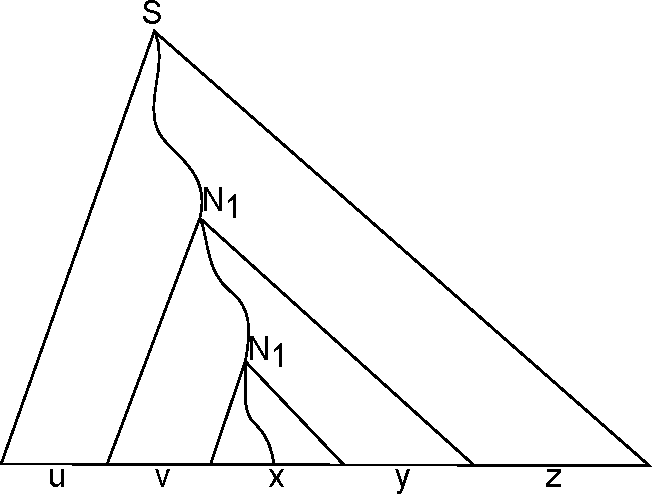
\includegraphics[width=0.5\textwidth]{figures/pumping_tree_1.pdf}
\caption{Разбиение цепочки для леммы о накачке}
\label{fig:pumping1}
\end{figure}

\begin{figure}
\centering
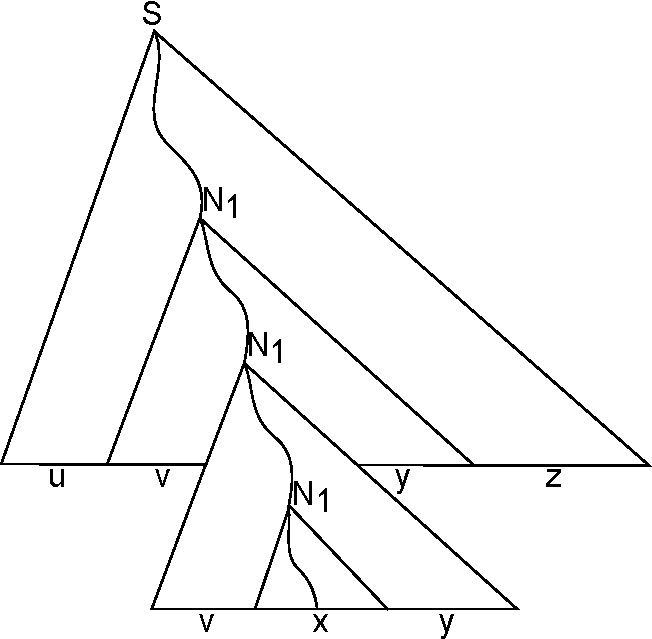
\includegraphics[width=0.5\textwidth]{figures/pumping_tree_2.pdf}
\caption{Пример накачки цепочки с рисунка~\ref{fig:pumping1}}
\end{figure}


\href{https://neerc.ifmo.ru/wiki/index.php?title=%D0%9B%D0%B5%D0%BC%D0%BC%D0%B0_%D0%BE_%D1%80%D0%B0%D0%B7%D1%80%D0%B0%D1%81%D1%82%D0%B0%D0%BD%D0%B8%D0%B8_%D0%B4%D0%BB%D1%8F_%D0%9A%D0%A1-%D0%B3%D1%80%D0%B0%D0%BC%D0%BC%D0%B0%D1%82%D0%B8%D0%BA}{Материалы по лемме о накачке для КС языков.}

Проверить неконтекстно-свободность языка $L=\{a^nb^nc^n \mid n>0\}$.

\section{Практика 5}

\subsection{Григорьев С.В.}

Преобразование в нормальную форму Хомского.

Формат входа:
\begin{enumerate}
\item Одна продукция на строку.
\item Продукция --- это список терминалов и нетерминалов через пробел, начинающийся с нереминала (левая часть продукции).
\item Нетерминалы --- заглавные буквы с опциональным числовым суффиксом.
\item Терминалы --- строчные буквы с опциональным числовым суффиксом.
\item Специальный символ \verb|eps| для обобзначения $\varepsilon$.
\end{enumerate}

Пример входя, описывающего граммтику $S \to a S b S \mid \varepsilon$:

\begin{verbatim}
S a S b S
S eps
\end{verbatim}

Домашнее задание.
\begin{enumerate}
    \item Реализовать преобразование в нормальную форму Хомского. На входе файл с граммтикой, на выходе --- файл с граммтикой в НФХ в том же формате, что и вход.
\end{enumerate}


\section{Лекция 6}

\subsection{Свойства замкнутости КС языков}

Глава 2.6 \href{https://github.com/YaccConstructor/articles/blob/master/InProgress/Formal_langs_CFPQ_course_notes/Formal_lang_CFPQ_course_notes.pdf}{конспекта}.

\subsection{Алгоритм CYK}

Глава 4.1 ``Алгоритм CYK'' \href{https://github.com/YaccConstructor/articles/blob/master/InProgress/Formal_langs_CFPQ_course_notes/Formal_lang_CFPQ_course_notes.pdf}{конспекта}.

\section{Практика 6}

\subsection{Григорьев С.В.}

Алгоритм CYK и алгоритм Хеллингса.

Формат входа для CYK:
\begin{enumerate}
\item Грамматика: смотри предыдущее ДЗ.
\item Входная строка: терминалы разделены пробелами.
\end{enumerate}

Пример входа, описывающего граммтику $S \to a S b S \mid \varepsilon$:

\begin{verbatim}
S a S b S
S eps
\end{verbatim}

Пример входной строки:
\begin{verbatim}
a a b a a b b b
\end{verbatim}


Формат входа алгоритма Хеллингса:
\begin{enumerate}
\item Грамматика: тот же формат, что и для CYK. НО! ИСпользуем преобразование а ослабленную НФХ.
\item Входной граф: файл в ктором на каждой строке записано ребро в виде тройки
$$
\langle\textit{вершина } \textit{метка\_ребра} \textit{ вершина}\rangle.
$$
Элементы тройки разделены пробелами.
\item Можно считать, что все вершины графа --- числа от нуля, идущие подряд.
\end{enumerate}

Пример входного графа:

\begin{center}
    \begin{tikzpicture}[node distance=3cm,shorten >=1pt,on grid,auto]
    \node[state] (q_0)   {$0$};
    \node[state] (q_1) [above right=of q_0] {$1$};
    \node[state] (q_2) [right=of q_0] {$2$};
    \node[state] (q_3) [right=of q_2] {$3$};
    \path[->]
    (q_0) edge  node {$a$} (q_1)
    (q_1) edge  node {$a$} (q_2)
    (q_2) edge  node {$a$} (q_0)
    (q_2) edge[bend left, above]  node {$b$} (q_3)
    (q_3) edge[bend left, below]  node {$b$} (q_2);
    \end{tikzpicture}
\end{center}

Пример описания входного графа:
\begin{verbatim}
0 a 1
1 a 2
2 a 0
2 b 3
3 b 2
\end{verbatim}

Домашнее задание.
\begin{enumerate}
    \item Реализовать алгоритм CYK для линейного входа. На вход принимаются два файла: с граммтикой и входной строкой. Результат (выводится ли входная цепочка в грамматике) печатается в консоль.
    \item Реализовать алгоритм Хеллингса. На вход принимается файл с граммтикой и файл с графом. В результирующий файл печатается граммтика в ослабленной НФХ (с которой непосредсвенно работал алгоритм) и множество пар достижимых вершин для стартового нетерминала (одна пара на строку, две вершины через пробел)
\end{enumerate}



\section{Лекция 7}

Алгоритмы решения задачи контекстно-свободной достижимости, основанные на операциях линейной алгебры.

\subsection{Алгоритм на основе матричного произведения}

Глава 5.1 \href{https://github.com/YaccConstructor/articles/blob/master/InProgress/Formal_langs_CFPQ_course_notes/Formal_lang_CFPQ_course_notes.pdf}{конспекта}.

\subsection{Алгоритм на основе тензорного произведения}

Глава 6 \href{https://github.com/YaccConstructor/articles/blob/master/InProgress/Formal_langs_CFPQ_course_notes/Formal_lang_CFPQ_course_notes.pdf}{конспекта}.

\section{Практика 7}

\subsection{Григорьев С.В.}

Алгоритмы на основе линейной алгебры.

Для реализации предлагается использовать следующие библиотеки. Так как с булевыми не везде хорошо, то будем использовать те типы, которые поддерживаются: \verb|Int|, \verb|float| и т.д.
\begin{itemize}
    \item Для языка Python --- \href{https://docs.scipy.org/doc/scipy/reference/sparse.html}{разреженные матрицы в scipy} и соответствующие опреации работы с ними: \href{https://docs.scipy.org/doc/scipy-0.14.0/reference/generated/scipy.sparse.kron.html}{\textbf{scipy.sparse.kron}} и \href{https://docs.scipy.org/doc/scipy/reference/generated/scipy.sparse.csr_matrix.html}{обычное матричное произведение}. Предпочтительный формат разреженных матриц --- CSR.
    \item Для языка Kotlin ---\href{http://la4j.org/}{la4j}. Операции: \href{http://la4j.org/apidocs/org/la4j/operation/ooplace/OoPlaceKroneckerProduct.html}{кронекер} и  \href{http://la4j.org/apidocs/org/la4j/operation/ooplace/OoPlaceMatricesMultiplication.html}{обычное умножение}.
\end{itemize}

Поэлементное сложение есть и там и там.

Для алгоритма на матричном умножении всё точно так же, как и в предыдущей ДЗ для Хеллингса.

Для тензорного произведения расширим формат представления входной грамматики.
Одна строка на нетерминал. Терминалы, нетерминалы, $\varepsilon$ обозначаются как и раньше.
Как и раньше, левая часть от правой отделена пробелом. В правой части можно использовать конструкции регулярных выражений: альтернатива, звезда клини, групперцющие скобки. Этот набор можно расширять по своему усмотрению.


Пример входа, описывающего граммтику $S \to (a S b)* \mid \varepsilon$:

\begin{verbatim}
S (a S b)* | eps
\end{verbatim}


Домашнее задание. Время на выполнение --- две недели. Один из алгоритмов --- на первую, оставшийся и эксперименты --- на вторую.
\begin{enumerate}
    \item Реализовать алгоритм, основанный на матричном умножении. На вход принимаются два файла: с граммтикой и входным графом. В результирующий файл печатается граммтика в ослабленной НФХ (с которой непосредсвенно работал алгоритм) и множество пар достижимых вершин для стартового нетерминала (одна пара на строку, две вершины через пробел).
    \item Реализовать алгоритм, основанный на тензорном произведении. На вход принимается файл с граммтикой и файл с графом. В результирующий файл печатается матрица смежности рекурсивного автомата (с которым непосредсвенно работал алгоритм, построчно, элементы разделены пробелом, пустая ячейка обозначается символом '.') и множество пар достижимых вершин для стартового нетерминала (одна пара на строку, две вершины через пробел).
    \item Сравнить производительность трёх реализованных алгоритмов (Хеллингс, матричное произведение, тензорное произведение). Результат --- описание эксперимента и таблица сравнения в readme.
\end{enumerate}



\section{Лекция 8}

Нисходящий синтаксический анализ: рекурсивный спуск и LL(k).


Глава 7, 8.1 и 8.2 \href{https://github.com/YaccConstructor/articles/blob/master/InProgress/Formal_langs_CFPQ_course_notes/Formal_lang_CFPQ_course_notes.pdf}{конспекта}.

\section{Практика 8}

\subsection{Григорьев С.В.}

Разработка синтаксических анализаторов: лексический и синтаксический анализы, абстрактный и конкретный синтаксис.

\subsubsection{Лексический анализ}

$$
E \to n \mid E \ + \ E \mid E \ * \ E
$$

Что такое $n$ (число)? Это абстракция.

$$
n = [1-9][0-9]^*
$$

$$
n = 0 \mid ((-)?[1-9][0-9]^*)
$$

$$
n = 0 \mid ((-)?[1-9][0-9]^*(.)[0-9]^*[1-9])
$$

То же самое верно и для других терминалов.

$$
E \to n \mid E \ op\_plus \ E \mid E \ op\_pow \ E \mid E \ op\_mult \ E
$$

$$
op\_pow = \verb|^|
$$


$$
op\_pow = **
$$

Для введени этой абстракции анализ языков разделяют на две стадии:
\begin{enumerate}
	\item Лексический анализ: переводим последовательность ``символов с клавиатуры'' в последовательность токенов/терминальных символов. Работает на основе регулярных выражений (как правило).

	\item Синтаксичексий анализ: переводим последовательность терминальных символов в структурное представление (дерево разбора). Работает на основе КС грамматик.
\end{enumerate}


Да, можно и не разделять: scanerless parsing.


\subsubsection{Абстрактный и конкретный синтаксис}

Структурное представление текста, удобное для решения тех или иных задач, не содержит многие детали исходного текста.

Абстрактное описание синтаксиса:
\begin{verbatim}
type stmt =
   ...
   | IfStmt of expr*List<stmt>*List<stmt>
   ...
\end{verbatim}

Примеры конкретного синтаксиса:
\hrule
\begin{verbatim}
...
if ( a + b > 0 )
then
  ...
else
  ...
...
\end{verbatim}
\hrule
\begin{verbatim}
...
if ( a + b > 0 )
{
  ...
}
else
{
  ...
}
...
\end{verbatim}
\hrule
\begin{verbatim}
...
cond_branch ( a + b > 0 )( ... )( ... )
...
\end{verbatim}
\hrule

Ещё пример абстрактного синтаксиса:

\begin{verbatim}
type arithExpr =
   | Num of int
   | OpPlus of arithExpr * arithExpr
   | OpMult of arithExpr * arithExpr
   | OpPow of arithExpr * arithExpr
\end{verbatim}

Важно то, что здесь нет ни слова про скобки, приоритеты, ассоциотивность.

\hrule
\begin{verbatim}
12 + 3 * 4 ^ 5 + 2
\end{verbatim}
\hrule
\begin{verbatim}
(12 + 3) * 4 ^ 5 + 2
\end{verbatim}
\hrule
\begin{verbatim}
12 + 3 * 4 ^ (5 + 2)
\end{verbatim}
\hrule
\begin{verbatim}
(12 + 3 * 4) ^ (5 + 2)
\end{verbatim}
\hrule

Потому что многие свойства естественным образом выражается структкрой дерева и, соответственно, детали исходного текста теряются.

\hrule
\begin{verbatim}
12 + 3 * 4 ^ 5 + 2

OpPlus
   (Num 12)
   (OpPlus
      (OpMult
         (Num 3)
         (OpPow
            (Num 4)
            (Num 5)))
      (Num 2)
\end{verbatim}
\hrule
\begin{verbatim}
(12 + 3) * 4 ^ 5 + 2

OpPlus
   (OpMult
      (OpPlus
         (Num 12)
         (Num 3))
      (OpPow
         (Num 4)
         (Num 5))
    (Num 2))
\end{verbatim}
\hrule
\begin{verbatim}
12 + 3 * 4 ^ (5 + 2)

OpPlus
   (Num 12)
   (OpMult
      (Num 3)
      (OpPow
         (Num 4)
         (OpPlus
            (Num 5)
            (Num 2))))
\end{verbatim}
\hrule
\begin{verbatim}
(12 + 3 * 4) ^ (5 + 2)

OpPow
   (OpPlus
      (Num 12)
      (OpMult
         (Num 3)
         (Num 4))
   )
   (OpPlus
      (Num 5)
      (Num 2))
\end{verbatim}
\hrule


Но важно помнить, что для разных задач нужна разная информация.


Можно начинать знакомство с \href{https://www.antlr.org/download.html}{ANTLR}, так как он будет использоваться в следующих домашних работах.



\section{Лекция 9}

Нисходящий синтаксический анализ: GLL и его применение для поиска путей с КС ограничениями.


Глава 8.3 и 8.4 \href{https://github.com/YaccConstructor/articles/blob/master/InProgress/Formal_langs_CFPQ_course_notes/Formal_lang_CFPQ_course_notes.pdf}{конспекта}.

\section{Практика 9}

\subsection{Григорьев С.В.}

Абстрактный и конкретный синтаксис языка запросов к графам, семантика языка запросов к гарфам.

Абстрактный синтаксис скрывает детали синтаксического анализа и конкретного ``текстового'' представления синтаксиса, оставляя только важную для дальнейшего анализа иформацию о структуре программы.

Первая, минималистичная, версия языка запросов к графам.

\begin{verbatim}
type script: Seq of List<stmt>

type stmt:
  | Connect of String
  | Select of obj_expr * graph_expr

type graph_expr =
  | Intersect of graph_expr * graph_expr
  | Query of pattern
  | GraphName of String

type obj_expr:
  | Edges
  | Count of obj_expr

type pattern:
  | smb of String
  | star of pattern
  | plus of pattern
  | alt of pattern * pattern
  | seq of pattern * pattern
  | option of pattern

\end{verbatim}

\newcommand{\sem}[1]{\llbracket #1 \rrbracket}

Тперь поговорим о семантике данного языка.

Семантика --- отображение из программ в семантический домен.
Программы обычно представляются как абстрактные синтаксические деревья.
Семантический домен --- то, что описывает смысл программы в контексте решаемой задачи.

Семантика бывает разной.
Классические примеры: динамическая семантика (вычисление программ) и статическая семантика (вывод типов).

Доменом динамической семантики арифметических выражений является множество функций из функции, сопоставляющей переменным целочисленные значения, в целые числа.

Семантика часто обозначается скобками $\llbracket$ и $\rrbracket$.

Семаника арифметических выражений:

$$\sem{\cdot} : (X \rightarrow \mathbb{N}) \rightarrow \mathbb{N}$$


\begin{align*}
  \sem{n}(\sigma) &= n, n \in \mathbb{N} \\
  \sem{v}(\sigma) &= \sigma(v) \\
  \sem{e_1 \oplus e_2}(\sigma) &= \sem{e_1}(\sigma) \otimes \sem{e_2}(\sigma) \\
  & \\
  \sem{-e}(\sigma) &= \sem{0-e}(\sigma)
\end{align*}

Здесь $\oplus$ --- конструкторы бинарных операций, $\otimes$ --- соответствующие арифметические функции.

В нашем случае, исполнение скрипта на получившимся языке достаточно естественно описывается состоянием из текущей базы данных, текущего графа, и текущего результата вычислений. Значение этой тройки и будут семантическим доменом нашего языка.

При обработке непустой последовательности инструкций сначала вычисляем результат выполнения первой инструкции, затем на нем --- всех остальных.

$$
\infer[]{c \xrightarrow{Seq \ (hd::tl)} c''}{c \xrightarrow{hd} c', \ \ c' \xrightarrow{Seq \ tl} c''}
$$

При обработке команды \verb|Connect| сохраняем её аргумент в конфигурации как путь к текущей базе данных.
$$
\infer[]{\langle db, graph, res\rangle \xrightarrow{Connect \ db'} \langle db', graph, res\rangle}{}
$$

При обработке инструкции \verb|Select| сперва вычисляется граф, из которого будут выбираться объекты, затем вычисляются сами объекты.

$$
\infer[]{c \xrightarrow{Select \ obj \ graph} c''}{c \xrightarrow{graph} c', \ \ c' \xrightarrow{obj} c''}
$$

При обработке инструкции \verb|Graph| загружаем в окружение граф из файла с именем, соотвествующим аргументу этой инструкции, лежащем в базе (директории), соответствующей значению \verb|cur_db|.

$$
\infer[]{\langle db, graph, res \rangle \xrightarrow{\textit{GraphName} \ name} \langle db ,loadGraph(String.concat(db,name)), res\rangle}{}
$$

При обработке инструкции \verb|Intersect| сперва вычисляем оба подвыражения, затем пересекаем получившиеся графы как конечные автоматы. Считаем все вершины стартовыми и финальными одновременно.

$$
\infer[]{\langle db, graph, res\rangle \xrightarrow{\textit{Intersect} \ graph_1 \ graph_2} \langle db, \textit{intersectFA}(graph', graph''), res\rangle}{\langle db, graph,res\rangle \xrightarrow{graph_1} \langle db, graph', res \rangle, \ \ \langle db, graph,res \rangle \xrightarrow{graph_2} \langle db, graph'', res \rangle}
$$


При обработке инструкции \verb|Query| необходимо построить минимальный детерминированный автомат по регулярному выражению, задаваемому шаблоном.

$$
\infer[]{\langle db, graph, res \rangle \xrightarrow{\textit{Query} \ pattern} \langle db, \textit{buildMinDFA}(pattern), res \rangle}{}
$$

При обработке инструкции \verb|Edges| в текущий результат вычислений записывается множество троек, соотвествующих рёбрам текущего графа.

$$
\infer[]{\langle db, graph, res \rangle \xrightarrow{\textit{Edges}} \langle db, graph, \{(v_i,e,v_j) \mid (v_i,e,v_j) \in graph.Edges\}\rangle}{}
$$

При обработке инструкции \verb|Count| сперва вычисляется подвыражене, а затем в текущий результат вычислений записывается размер результата вычисления подвыражения, если результат был множеством.

$$
\infer[type\_of(res') \equiv Set ]{\langle db, graph, res \rangle \xrightarrow{\textit{Count} \ expr} \langle db, graph, Set.count(res') \rangle}{\langle db, graph, res \rangle \xrightarrow{expr} \langle db, graph, res' \rangle}
$$

--------------------------------------------------------------------------------




Расширенная версия.

\begin{verbatim}
type script = Seq of List<stmt>

type stmt =
  | Connect of String
  | NamedPattern of String * pattern
  | Select of obj_expr * graph_expr

type graph_expr =
  | Intersect of graph_expr * graph_expr
  | Query of pattern
  | GraphName of String
  | SetStartAndFinal of vertices * vertices * graph_expr

type vertices =
  | Set of Set<int>
  | Range of int * int
  | None

type obj_expr =
  | Edges
  | Filter of cond * obj_expr
  | Count of obj_expr

type cond =
  | Cond of String * String * String * bool_expr

type bool_expr =
  | LblIs   of String * String
  | IsStart of String
  | IsFinal of String
  | And of bool_expr * bool_expr
  | Or of bool_expr * bool_expr
  | Not of bool_expr

type pattern =
  | Term of String
  | Nonterm of String
  | Star of pattern
  | Plus of pattern
  | Alt of pattern * pattern
  | Seq of List<pattern>
  | Option of pattern

\end{verbatim}


Для описания семантики для добавленных конструкций потребуется изменить домен --- в него необходимо добавить grammar (текущую граммтику).


При обработке инструкции \verb|NamedPattern| добавляем в \textit{grammar} правило, где левая часть --- имя шаблона, а правая часть --- регулятрное выражение построенное по шаблону.

$$
\infer[]{\langle db, graph, grammar, res \rangle \xrightarrow{\textit{NamedPattern} \ name \ pattern} \langle db, graph, \textit{addRule(grammar, name, pattern)}, res \rangle}{}
$$

Так как теперь запрос может быть не только регулярным, то изменится обработка кинструкции \verb|Query|. Теперь вместо детерминированного конечного автомата строится рекурсивный конечный автомат с учётом накопленной грамматики.

$$
\infer[]{\langle db, graph, grammar, res \rangle \xrightarrow{\textit{Query} \ pattern} \langle db, \textit{buildRSM}(pattern, grammar), grammar, res \rangle}{}
$$

Как следствие, изменяется обработка инструкции \verb|Intersect|: нам необхоимо отслеживать, какого типа графы пересекаются, так как для успешного выполнения операции необходимо, чтобы хотя бы один из них был обыкновенным конечным автоматом.

$$
\infer[\textit {$g'$ is DFA or $g''$ is DFA}]{\langle db, g, grm, res\rangle \xrightarrow{\textit{Intersect} \ g_1 \ g_2} \langle db, \textit{intersect}(g', g''), grm, res\rangle}{\langle db, g, grm, res\rangle \xrightarrow{g_1} \langle db, g', grm, res \rangle, \ \ \langle db, g, grm, res \rangle \xrightarrow{g_2} \langle db, g'', grm, res \rangle}
$$

Добавим операцию, позволяющую явно указывать стартовые и финальные состояния \verb|SetStartAndFinal|.

{
\scriptsize
$$
\infer[res' \neq \varnothing, res'' \neq \varnothing]{\langle db, g, grm, res\rangle \xrightarrow{\textit{SetStartAndFinal} \ start \ final \ g_1} \langle db, \textit{(g' with Start = $res'$, Final = $res''$)}, grm, res\rangle}{\langle db, g, grm, res\rangle \xrightarrow{g_1} \langle db, g', grm, res \rangle, \ \ \langle db, g', grm, res \rangle \xrightarrow{start} \langle db, g', grm, res' \rangle, \ \ \langle db, g', grm, res \rangle \xrightarrow{final} \langle db, g', grm, res'' \rangle}
$$
}

{
\scriptsize
$$
\infer[res' = \varnothing, res'' \neq \varnothing]{\langle db, g, grm, res\rangle \xrightarrow{\textit{SetStartAndFinal} \ start \ final \ g_1} \langle db, \textit{(g' with Final = $res''$)}, grm, res\rangle}{\langle db, g, grm, res\rangle \xrightarrow{g_1} \langle db, g', grm, res \rangle, \ \ \langle db, g', grm, res \rangle \xrightarrow{start} \langle db, g', grm, res' \rangle, \ \ \langle db, g', grm, res \rangle \xrightarrow{final} \langle db, g', grm, res'' \rangle}
$$
}

{
\scriptsize
$$
\infer[res' \neq \varnothing, res'' = \varnothing]{\langle db, g, grm, res\rangle \xrightarrow{\textit{SetStartAndFinal} \ start \ final \ g_1} \langle db, \textit{(g' with Start = $res$)}, grm, res\rangle}{\langle db, g, grm, res\rangle \xrightarrow{g_1} \langle db, g', grm, res \rangle, \ \ \langle db, g', grm, res \rangle \xrightarrow{start} \langle db, g', grm, res' \rangle, \ \ \langle db, g', grm, res \rangle \xrightarrow{final} \langle db, g', grm, res'' \rangle}
$$
}


{
\scriptsize
$$
\infer[res' = \varnothing, res'' = \varnothing]{\langle db, g, grm, res\rangle \xrightarrow{\textit{SetStartAndFinal} \ start \ final \ g_1} \langle db, g', grm, res\rangle}{\langle db, g, grm, res\rangle \xrightarrow{g_1} \langle db, g', grm, res \rangle, \ \ \langle db, g', grm, res \rangle \xrightarrow{start} \langle db, g', grm, res' \rangle, \ \ \langle db, g', grm, res \rangle \xrightarrow{final} \langle db, g', grm, res'' \rangle}
$$
}

$$
\infer[]{\langle db, graph, grammar, res \rangle \xrightarrow{\textit{Set} \ s} \langle db, g, grammar, s \cap \textit{graph.Vertices} \rangle}{}
$$


$$
\infer[]{\langle db, graph, grammar, res \rangle \xrightarrow{\textit{None}} \langle db, g, grammar, \varnothing \rangle}{}
$$

$$
\infer[]{\langle db, graph, grammar, res \rangle \xrightarrow{\textit{Range} \ x \ y} \langle db, g, grammar, \textit{graph.Vertices} \cap \{ \min(x,y) \ldots \max(x,y)\} \rangle}{}
$$

Расширим возможности обработки результата пересечения. Для этого добавим фильтрацию рёбер. Обработка конструкции \verb|Filter| выглядит следующим образом.

$$
\infer[\textit{type of res' is Set<Edge>}]{\langle db, graph, grammar, res \rangle \xrightarrow{\textit{Filter} \ cond \ src} \langle db, g, grammar, \textit{Set.filter cond res'} \rangle}{\langle db, graph, grammar, res \rangle \xrightarrow{src} \langle db, g, grammar, res' \rangle}
$$



\section{Лекция 10}

Восходящий синтаксический анализ: алгоритмы семейства LR.


Глава 9.1 \href{https://github.com/YaccConstructor/articles/blob/master/InProgress/Formal_langs_CFPQ_course_notes/Formal_lang_CFPQ_course_notes.pdf}{конспекта}.

\section{Практика 10}

\subsection{Григорьев С.В.}


Синтаксический анализ с использованием генератора синтаксических анализаторов ANTLR.

Домашняя страница \href{https://www.antlr.org/index.html}{ANTLR}.

\href{https://github.com/antlr/antlr4/blob/master/doc/python-target.md}{ANTLR для Python}.


\href{https://github.com/antlr/antlr4/blob/master/doc/java-target.md}{ANTLR для Java}.


Задача на дом.
\begin{enumerate}
  \item Реализовать синтаксический анализатор языка запросов к графовым БД (разработанный в рамках предыдущей ДЗ) с использованием ANTLR (или другого инструмента создания синтаксических анализаторов). Ожидаемая функциональность следующая.
  \begin{itemize}
  \item Чтение скрипта из файла.
  \item Чтение скрипта с консоли.
  \item Вывод в консль сообщения о корректности/некорректности скрипта.
  \item Вывод в файл дерева разбора скрипта в формате GraphViz/DOT.
  \end{itemize}
\end{enumerate}



\section{Лекция 11}

Восходящий синтаксический анализ: алгоритмы семейства LR.


Глава 9.2 \href{https://github.com/YaccConstructor/articles/blob/master/InProgress/Formal_langs_CFPQ_course_notes/Formal_lang_CFPQ_course_notes.pdf}{конспекта}.

\section{Практика 11}

\subsection{Григорьев С.В.}


Исполнение скриптов запросов.

\href{https://packages.ubuntu.com/search?keywords=antlr4}{ANTLR-пакет для Ubuntu}.

\href{https://github.com/shmatov/antlr4-calculator}{Пример калькулятора}.


Задача на дом.
\begin{enumerate}
  \item Автоматизированная сборка с генерацией файлов по грамматике. Сгенерированные файлы удалены из репозитория.
  \item Поддержка выполнения части команд языка запросов. На данном этапе считаем, что скрипт полностью корректен.
  \begin{itemize}
    \item \verb|connect| полностью
    \item \verb|list| полностью
    \item \verb|named_pattern| можно без конструкций регулярных выражений (звезда Клини, альтернатива)
    \item \verb|select| можно только \verb|exists| и \verb|v_expr| только имя (\verb|name of String|)
  \end{itemize}
  \item Тесты. Очень много тестов. Каждая смысловая конструкция должна бять проверена.

\end{enumerate}



\section{Лекция 12}

Контрольная работа по КС языкам.

\section{Практика 12}

\subsection{Григорьев С.В.}


Исполнение скриптов запросов.

\href{https://packages.ubuntu.com/search?keywords=antlr4}{ANTLR-пакет для Ubuntu}.

\href{https://github.com/shmatov/antlr4-calculator}{Пример калькулятора}.


Задача на дом.
\begin{enumerate}
  \item Полная поддержка языка запросов.
  \item Тесты. Очень много тестов. Каждая смысловая конструкция должна бять проверена.

\end{enumerate}


\section{Лекция 13}

Сиинтаксически управляемая трансляция, атрибутные граммтики.

\href{https://github.com/YaccConstructor/articles/blob/master/InProgress/Formal_languages_course/attrib_grammars/presentation.pdf}{Презентация}.

\section{Практика 11}

\subsection{Григорьев С.В.}


Дополнительные задачи на зачёт.

Для получения зачёта необходимо выполнить следующие условия.

\begin{enumerate}
\item Сдасть все семестровые задачи.
\item Если какие-то из задач в семестре были сданы с нарушением условий, установленных в начаое семестра, то необходимо решить дополнительные задачи. Какие именно, указано в \href{https://docs.google.com/spreadsheets/d/1g1ZVACS0ATW7pVpvSI6L4mLKsxyuJEVh_HX6xhQRdmI/edit#gid=0}{таблице с результатами}, в колонке ``Доп. задача''.
\end{enumerate}

Дополнительные задачи. В таблице указаны их номера. Красным выделены те, которые нужно решить.
Для каждой задачи должно быть представлено:
\begin{itemize}
	\item Расширение абстрактного синтаксиса (добавлено в документацию в репозитории)
	\item Расширенеи конкретного синтаксиса (расширена документация в репозитории)
	\item Примеры (добавлено в документацию в репозитории)
	\item Реализация
	\item Тесты
\end{itemize}
\begin{enumerate}
  \item Расширить команду \verb|list| так, чтобы можно было опционально указывать путь к БД, графы в которой хочется вывести. По умолчанию всё так же выводятся графы из текущей БД.
  \item Расширить команду \verb|list| так, чтобы с её помощью можно было вывести множество различных меток рёбер в указанном графе.

  \item Расширить команду \verb|select| возможностью опционально указывать алгоритм, с помощью которого выполнять текущий запрос. Воспроизвести эксперимент из ДЗ 5. Повлияло ли использование языка запросов на результаты экспериментов?

  \item Расширить команду \verb|select| возможностью в качестве графа-источника использовать результат операций объединения, пересечения и допллнения графов из текущей базы данных. То есть во \verb|from| можно птсать выражение над графами типа \verb|from| $\overline{(g_1 \cup g_2)} \cap g_3$. Данные операции должны трпктоваться как операции над языками, задаваемыми автоматом, где переходы определяются графом, а стартовые и финальные состояния --- все вершины графа.


\end{enumerate}



\bibliographystyle{abbrv}
\bibliography{Formal_language_course}


\end{document}
